We show the evaluation of our NAT system in this section.
SW and HW NAT implementation are considered (referred to as SW NAT and HW NAT). Two ablation settings (HW NAT without translation, without NAT) are introduced to measure the overhead of our HW NAT design.
With four settings above, we do two evaluations:
\begin{itemize}
    \item We measure the throughput with different packet sizes from 0 to 5000 bytes.
    \item We measure the throughput with different numbers of connections from 0 to 1024.
\end{itemize}

% with two dimension (different packet sizes and different numbers of connections).





% \textbf{We do not measure the latency.} HW NAT introduces minimal latency overhead compared to no NAT. The overhead is predictable, averaging only a few cycles. The maximum value ?? accounts for only a small fraction (??\%) of the total latency. And since the average latency is very small, we could not measure it accurately with our devices.

\subsection{Evaluation Setting}

We detail our settings in two evaluations here. The connection hash table size is configured as 1024 for both evaluations. A traffic generator written in C language continuously sends TCP packets to the desktop machine via a Linux packet socket to the 10GbE interface of the board, which will flow through PL, in an infinite loop. The throughput is measured by dividing the data amount over the time of sending it. The data amount is set to 100 gigabits.
The details of the four settings are:

\begin{itemize}
    \item {\textbf{HW NAT}}: Our design stated in System Design and Implementation sections. It is a hardware-based NAT system that uses our custom NAT IP core, which can intercept the communication between MAC/GTH and DMA, and modify the IP and TCP headers of the packets according to the NAT rules. It uses a bidirectional hash table to store the mappings of LAN 5 tuple and WAN 5 tuple, and uses XOR as the hash function, and linear probing as the collision resolution strategy. It can achieve high-speed data conversion and forwarding, and improve the throughput.
    \item {\textbf{SW NAT}}: A software-based NAT system that runs on four threads and uses a shared hash table with linear probing. The table size is also 1024. It can be considered as a baseline compared to our HW NAT.
    \item {\textbf{HW NAT w/o translate}}: The same as \textbf{HW NAT}, but we use packets that do not need to translate (e.g. ICMP packets) to measure the performance.
    \item {\textbf{w/o NAT}}: No NAT at all, packets are directly forwarded between MAC/GTH and DMA. This is the ideal scenario and can be used as an upper bound to evaluate the performance of our system.
\end{itemize}

\subsection{Result}

\begin{figure}
    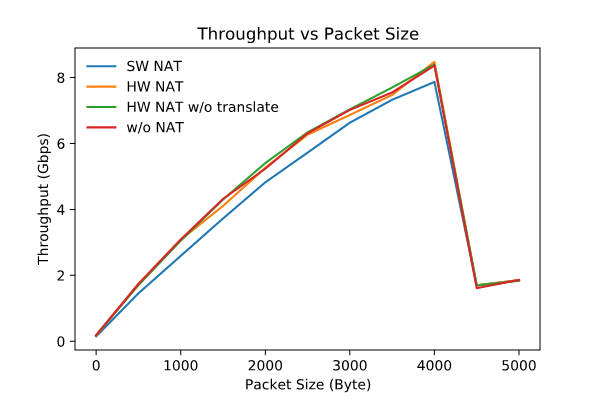
\includegraphics[width=\linewidth]{images/Result1.png}
    \caption{Result1}
    \Description{1}
\end{figure}

Figure 1?? shows the relationship between throughput and packet size. As the packet size increases, the throughput also increases, until it reaches a maximum value at around 4000 bytes, and then suddenly drops. This phenomenon is observed for all scenarios.

\begin{figure}
    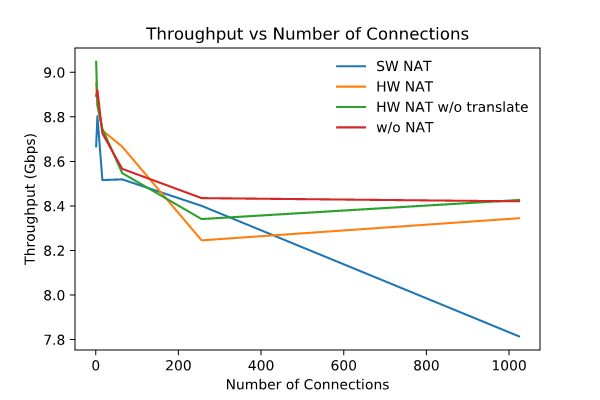
\includegraphics[width=\linewidth]{images/Result2.png}
    \caption{Result2}
    \Description{2}
\end{figure}

Figure 2?? shows the relationship between throughput and number of connections. As the number of connections increases, the throughput of SW NAT drops sharply, while the throughput of other scenarios remains stable. 

\subsection{Interpretation}

In Figure 1??, we can see that SW NAT has a performance gap with no NAT, indicating that SW NAT is a bottleneck that degrades the overall system performance. We can also see that HW NAT has a performance improvement compared to SW NAT, indicating that hardware implementation has better performance than software. And there's almost no performance gap between HW NAT and no NAT, which indicates that hardware implementation has little impact on the original system performance.

Figure 2?? shows that SW NAT does not scale well with the number of connections, due to the CPU overhead of software NAT and the synchronization overhead of sharing the NAT table. On the other hand, HW NAT scales well with the number of connections, as it uses a bidirectional hash table and the arbiter design to handle the NAT mappings.

\subsection{Anomalies}
There are two anomalies in our evaluation results. We try to give some speculative guesses about them.

\textbf{Why does the packet size need to be large to achieve line rate?} We speculate that this is due to the poor performance of the ARM cores and the not-so-good performance of DMA, MAC, and GTH IP. The FPGA side has to process the packets at a high speed, and may not be able to handle the small packets efficiently. Therefore, the packet size needs to be large enough to saturate the bandwidth of the FPGA side.

\textbf{Why is there a cliff-like drop after 4000 bytes?} We speculate that this is due to the existence of a 4K buffer in the link, which may cause extra overflow handling for large packets. When the packet size exceeds 4K, the buffer may not be able to store the whole packet and may have to split it into multiple segments, which may incur additional overhead and reduce the throughput.



